\documentclass[tikz]{standalone}
\usepackage{fourier}
\usepackage{tikz}

\begin{document}
	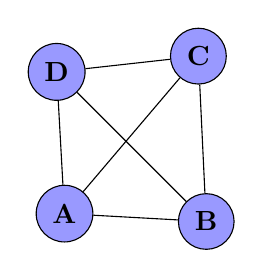
\begin{tikzpicture}
		\node[draw,circle,fill=blue!40!white](a) at (0.1,0.1) {\textbf{A}};
		\node[draw,circle,fill=blue!40!white](b) at (1.9,0) {\textbf{B}};
		\node[draw,circle,fill=blue!40!white](c) at (1.8,2.1) {\textbf{C}};
		\node[draw,circle,fill=blue!40!white](d) at (0,1.9) {\textbf{D}};
		\draw (a)--(b) (b)--(c) (c)--(d) (d)--(a) (a)--(c) (b)--(d);
	\end{tikzpicture}
\end{document}
